\documentclass[14pt,compress]{beamer}
\usepackage[spanish]{babel}
\usepackage[utf8]{inputenc}
\usepackage{presento}
\usepackage{comment}

\makeatletter
\newcommand{\vast}{\bBigg@{5}}
\newcommand{\Vast}{\bBigg@{6}}
\makeatother

%configuration file
%\setbeamercolor{title}{fg=DarkRed}
%\setbeamercolor{frametitle}{fg=DarkRed}
\setbeamercolor{normal text}{fg=darkgray}
\usebeamercolor[fg]{normal text}
%\setbeamercolor{block title}{fg=black,bg=Fern!25!white}
%\setbeamercolor{block body}{fg=black,bg=Fern!25!white}
%\setbeamercolor{alerted text}{fg=AlertColor}
%\setbeamercolor{itemize item}{fg=Charcoal}

\usepackage[font={color=dimgray},figurename={ },labelfont={ }]{caption}

% personal data
\newcommand{\mycongress}{\setnote{\color{darkgray}\small
I Encuentro Nacional de Din\'amica Cu\'antica en la Materia}}
\newcommand{\myTitle}{\color{orange}{\fontsize{27}{29}\selectfont 
Implementación de Métodos de Aprendizaje Automatizado
en problemas colisionales}}
\newcommand{\myemail}{\setnote{\color{darkgray}\scriptsize 
alemendez@iafe.uba.ar}}
\newcommand{\myDetails}{\setnote{\color{darkgray}\small 
1 de Septiembre -- Buenos Aires}}

% colors: black, blue, brown, cyan, darkgray, gray, green, 
% lightgray, lime, magenta, olive, orange, pink, purple, red, teal, 
% violet, white, yellow.

\begin{document}
%%%%%%%%%%%%%%%%%%%%%%%%%%%%%%%%%%%%%%%%%%%%%%%%%%%%%%%%%%%%%%%%%
\begin{frame}[plain]
\vfill
\mycongress

\vspace{0.7cm}
\myTitle
% \hline

\noindent\makebox[\linewidth]{\rule{0.85\paperwidth}{0.7pt}}
\vfill

% \vspace{0.5cm}
\hspace{2.75cm}\text{\color{teal}{\normalsize Alejandra Mendez,}} \\
\hspace{2.75cm}\text{\color{teal}{\normalsize Juan Di Filippo,}} \\
\hspace{2.75cm}\text{\color{teal}{\normalsize Sebasti\'an L\'opez,}} \\
\hspace{2.75cm}\text{\color{teal}{\normalsize Dar\'io Mitnik,}} \\
\vfill
\vspace{-0.25cm}
\hspace{2.5cm}\myemail
\vfill
\begin{tikzpicture}[remember picture,overlay]
\node[xshift=-10.7cm,yshift=-6.45cm] at (current page.north east) 
{
\includegraphics[width=0.28\textwidth]{iafe.jpg}};
\end{tikzpicture}

\vspace{-0.5cm}
\centering
\myDetails 

\end{frame}
\begin{comment}
%%%%%%%%%%%%%%%%%%%%%%%%%%%%%%%%%%%%%%%%%%%%%%%%%%%%%%%%%%%%%%%%%%%%%%%%
\section{Machine Learning}
%%%%%%%%%%%%%%%%%%%%%%%%%%%%%%%%%%%%%%%%%%%%%%%%%%%%%%%%%%%%%%%%%%%%%%%%
\framepic[1.]{figures/mlcover_modif.png}{
 \begin{textblock}{8}(6.5,-2.2)
    {\color{orange0}
\text{\huge \bf Machine} \\
\vspace{2pt}
\text{\huge\bf Learning}}
 \end{textblock} }
%%%%%%%%%%%%%%%%%%%%%%%%%%%%%%%%%%%%%%%%%%%%%%%%%%%%%%%%%%%%%%%%%%%%%%%%
\section{Inferencia Bayesiana}
%%%%%%%%%%%%%%%%%%%%%%%%%%%%%%%%%%%%%%%%%%%%%%%%%%%%%%%%%%%%%%%%%%%%%%%%
\begin{frame}
\frametitle{Optimización Bayesiana}

Sea $f:\mathcal{X}\rightarrow\mathbb{R}$
\begin{equation*}
  \mathbf{x}_{\mbox{\scriptsize opt}}=
  \underset{\mathbf{x}\in\mathcal{X}}{\mbox{arg máx}} f(\mathbf{x})
\end{equation*}
\begin{flushright}
donde $\mathcal{X}\subset\mathbb{R}^d $
\end{flushright}

\pause
\begin{equation*}
\tikzmarkin[draw=darkgray,fill=darkgray!10]{bayes}(0.2,-0.6)(-0.1,0.85)
p(\boldsymbol{\theta}|\mathbf{y},X)=
\frac{p(\mathbf{y}|X,\boldsymbol{\theta})p(\boldsymbol\theta)}
{p(\mathbf{y}|X)}
\tikzmarkend{bayes}
\end{equation*}

\end{frame}
%%%%%%%%%%%%%%%%%%%%%%%%%%%%%%%%%%%%%%%%%%%%%%%%%%%%%%%%%%%%%%%%%%%%%%%%
\begin{frame}
\frametitle{Procesos Gaussianos}

Un proceso Gaussiano es un proceso estocástico especificado por

\begin{itemize}
\item Función media: 
\begin{equation*}
\mu(\mathbf{x})=\mathbb{E}\left[f(\mathbf{x})\right]
\end{equation*}
\item Función de covariancia:
\begin{equation*}
\kappa(\mathbf{x},\mathbf{x}')=\mathbb{E}\left[
\left(f(\mathbf{x})-\mu(\mathbf{x})\right)
\left(f(\mathbf{x}')-\mu(\mathbf{x}')\right)\right]
\end{equation*}
\end{itemize}

\end{frame}
%%%%%%%%%%%%%%%%%%%%%%%%%%%%%%%%%%%%%%%%%%%%%%%%%%%%%%%%%%%%%%%%%%%%%%%%
\begin{frame}
\frametitle{Formalismo}

In supervised learning, we often use parametric models 
$p(\mathbf{y} \lvert \mathbf{X},\boldsymbol\theta)$ to explain data 
and infer optimal values of parameter $\boldsymbol\theta$ via 
maximum likelihood or maximum a posteriori estimation.
If needed we can also infer a full posterior distribution
$p(\boldsymbol\theta \lvert \mathbf{X},\mathbf{y})$ instead of a 
point estimate $\boldsymbol{\hat\theta}$. 
With increasing data complexity, models with a higher number of 
parameters are usually needed to explain data reasonably well. 
Methods that use models with a fixed number of parameters are called 
parametric methods. 

In non-parametric methods, on the other hand, the number of parameters depend on the dataset size. For example, in [Nadaraya-Watson kernel regression](https://en.wikipedia.org/wiki/Kernel_regression), a weight $w_i$ is assigned to each observed target $y_i$ and for predicting the target value at a new point $\mathbf{x}$ a weighted average is computed: 

$$f(\mathbf{x}) = \sum_{i=1}^{N}w_i(\mathbf{x})y_i$$

$$w_i(\mathbf{x}) = \frac{\kappa(\mathbf{x}, \mathbf{x}_{i})}{\sum_{i'=1}^{N}\kappa(\mathbf{x}, \mathbf{x}_{i'})}$$

Observations that are closer to $\mathbf{x}$ have a higher weight than observations that are further away. Weights are computed from $\mathbf{x}$ and observed $\mathbf{x}_i$ with a kernel $\kappa$. A special case is k-nearest neighbors (KNN) where the $k$ closest observations have a weight $1/k$, and all others have weight $0$. Non-parametric methods often need to process all training data for prediction and are therefore slower at inference time than parametric methods. On the other hand, training is usually faster as non-parametric models only need to remember training data. 


\end{frame}
%%%%%%%%%%%%%%%%%%%%%%%%%%%%%%%%%%%%%%%%%%%%%%%%%%%%%%%%%%%%%%%%%%%%%%%%
\begin{frame}
\frametitle{Tipos de kernels}

\begin{itemize}
\item Lineal:
\item Polinomico: 
\item Gaussiano:
\item Exponencial:
\item Laplaciano:
\item Tangente hiperbólico:
\end{itemize}

\end{frame}
%%%%%%%%%%%%%%%%%%%%%%%%%%%%%%%%%%%%%%%%%%%%%%%%%%%%%%%%%%%%%%%%%%%%%%%%
\begin{frame}
\frametitle{La función de adquisición}


\end{frame}
\end{comment}
%%%%%%%%%%%%%%%%%%%%%%%%%%%%%%%%%%%%%%%%%%%%%%%%%%%%%%%%%%%%%%%%%%%%%%%%
%%%%%%%%%%%%%%%%%%%%%%%%%%%%%%%%%%%%%%%%%%%%%%%%%%%%%%%%%%%%%%%%%%%%%%%%
\framepic[1.]{figures/ionization.png}{}
%%%%%%%%%%%%%%%%%%%%%%%%%%%%%%%%%%%%%%%%%%%%%%%%%%%%%%%%%%%%%%%%%%%%%%%%
\section{DIM}
%%%%%%%%%%%%%%%%%%%%%%%%%%%%%%%%%%%%%%%%%%%%%%%%%%%%%%%%%%%%%%%%%%%%%%%%
\begin{frame}
\frametitle{Método de Inversión Depurada (DIM)}

\vspace{-1.5cm}
\begin{equation*}
\tikzmarkin[draw=darkgray,fill=darkgray!10]{potencial}(0.2,-0.3)(-0.1,0.65)
T_{fi} = \big| \langle \psi_f |  V 
| \psi_i \rangle \big|^2 
\tikzmarkend{potencial}
\end{equation*}
\begin{tikzpicture}[remember picture, overlay,
  expl1/.style={draw=red,fill=orange!7,rounded corners,text width=3cm,
  minimum width=1.2cm, minimum height=0.7cm, text centered},
  arrow/.style={red,ultra thick,->,>=latex}
  ]
\node<2->[expl1] (potexp) at (9.5cm,2cm) {\color{orange-red}{¿Cómo conocemos V?}};
\draw<2->[arrow, bend right=30, dashed] ([xshift=0cm,yshift=0cm]{potexp.west}) to
         ([xshift=2.5cm,yshift=-0.2cm]{potencial});  
\node<3> (schro) at (5cm,-1cm)
{$ \left[ -\frac{1}{2} \frac{d^2}{d r^2} + \frac{l(l+1)}{2 r^2} 
+ V_{nl}(r) \right] \, P_{nl}(r) = 
E_{nl} \, P_{nl}(r) $};
\node<4-> (schro) at (5cm,-1cm)
{$ \left[ -\frac{1}{2} \frac{d^2}{d r^2} + \frac{l(l+1)}{2 r^2} 
- \frac{Z_{nl}(r)}{r} \right] \, P_{nl}(r) = 
E_{nl} \, P_{nl}(r) $};
\node<5-> (znl) at (5cm,-2.5cm)
{$ Z_{nl}(r) = -\frac{1}{2} 
\frac{P_{nl}''(r)}{ P_{nl}(r)} \,r
+ \frac{l(l+1)}{2 r} - E_{nl} \,r $};
\end{tikzpicture}

\end{frame}
%%%%%%%%%%%%%%%%%%%%%%%%%%%%%%%%%%%%%%%%%%%%%%%%%%%%%%%%%%%%%%%%%%%%%%%%
\begin{frame}
\frametitle{Houston, we have a problem!}

\vspace{-0.25cm}
\begin{tikzpicture}
  \node (img1) 
  {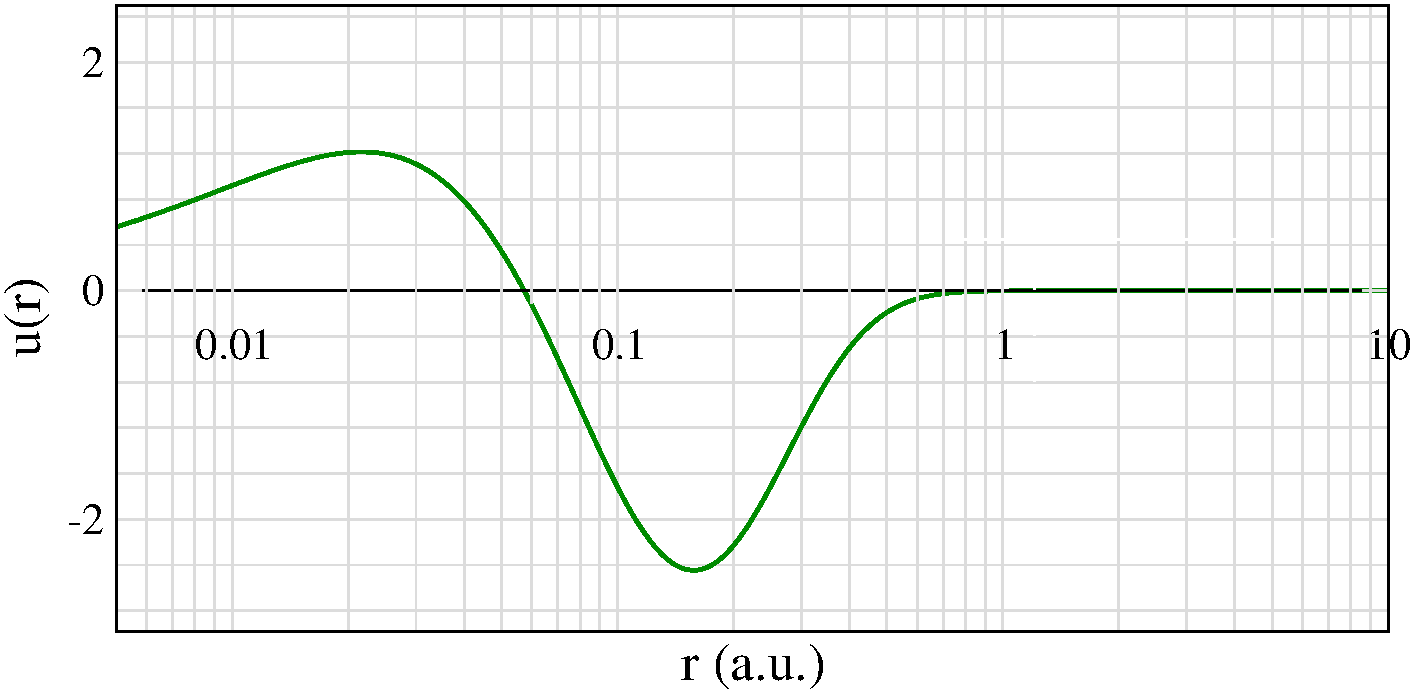
\includegraphics[width=0.95\textwidth]{figures/dim/wavefun2sKr.pdf}};
  \node<1-> (eq1) at (img1) [yshift=1.4cm,xshift=1.5cm]
  {$Z(r) = -\frac{1}{2} \frac{P''(r)}{P(r)} \,r  - E \, r$}; 
  \node (eq2) at (img1) [yshift=3cm,xshift=4cm] 
  {{\normalsize $2s$ Kr}}; 
  \node<2-> (img2) at (img1.west) [xshift=2cm,yshift=-2.25cm]
  {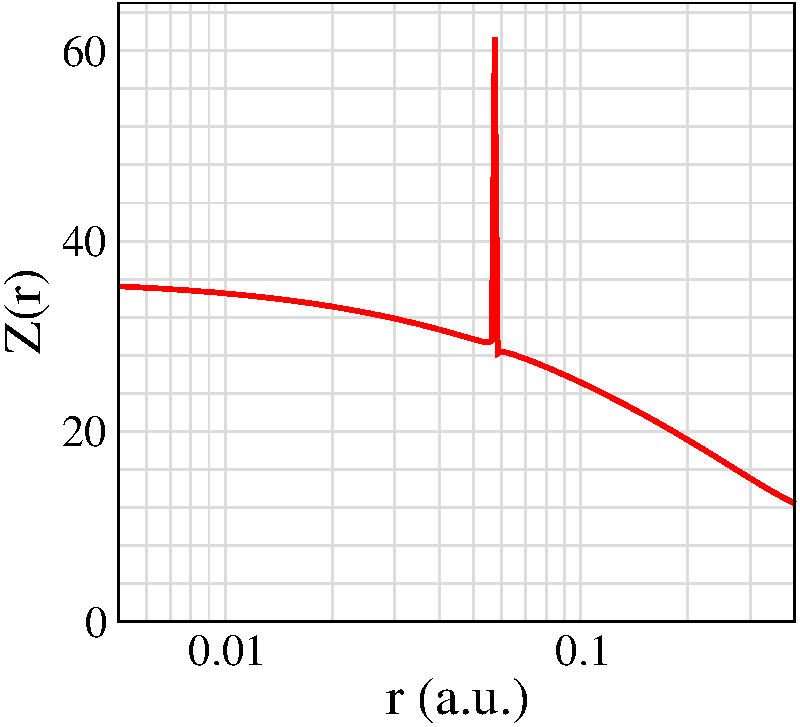
\includegraphics[width=0.4\textwidth]{figures/dim/problem1-2sKr.pdf}};
  \node<3-> (img3) at (img1.east) [xshift=-1.75cm,yshift=-2.25cm]
  {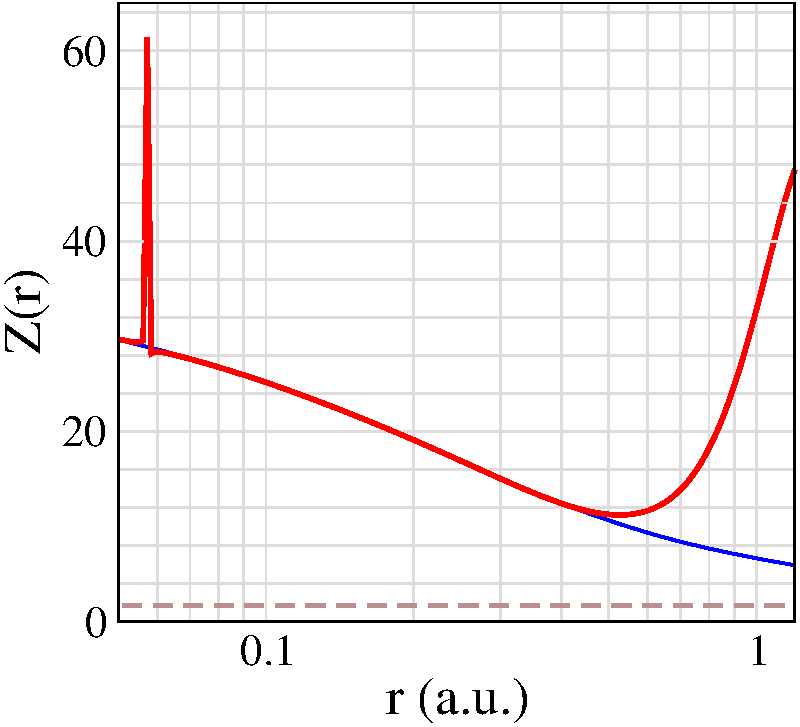
\includegraphics[width=0.4\textwidth]{figures/dim/problem2-2sKr.pdf}};
\end{tikzpicture}

\end{frame}
%%%%%%%%%%%%%%%%%%%%%%%%%%%%%%%%%%%%%%%%%%%%%%%%%%%%%%%%%%%%%%%%%%%%%%%%
\begin{frame}
\frametitle{Depuraci\'on}

\begin{tikzpicture}[remember picture,overlay]
  \tikzset{shift={(current page.center)}}%xshift=-1.5cm,yshift=0cm}
  \node (img1) 
  {\includegraphics[width=0.7\textwidth]{figures/dim/depuration2sN-a.eps}};
  \node (name) at (img1) [yshift=2.9cm,xshift=2.8cm] 
  {$2s$ N};
  \node<3-> (eq1) at (img1) [yshift=-3.5cm,xshift=0cm]
  {$\tikzmarkin[draw=orange,fill=orange!10]{depuration}(0.2,-0.5)(-0.1,0.65)
   Z(r) = 1+\sum_{j} \alpha_j e^{-\beta_j r} 
   \tikzmarkend{depuration}$};
  \node<3-> (img2) 
  {\includegraphics[width=0.7\textwidth]{figures/dim/depuration2sN-b.eps}};
  \node<2-> (asym) at (img1) [yshift=0cm,xshift=-1.1cm]
  { {\small $\Bigg\{ \!\! \begin{array}{c}
  \!\!\!\!Z_N :\, r=0 \\ 
  \,1 \,\,\,:\, r\rightarrow \infty\\ \end{array} $ } };
  \node<4-> (eq1) at (img1) [yshift=-3.5cm,xshift=0cm]
  {$\tikzmarkin[draw=orange,fill=orange!10]{depuration}(0.21,-0.5)(-0.1,0.65)
   Z(r) = 1+\sum_{j} {\color{orange}{\mathbf{\boldsymbol\alpha_j}}} 
          e^{-{\color{orange}{\mathbf{\boldsymbol\beta_j}}} r} 
   \tikzmarkend{depuration}$};
\end{tikzpicture}

\end{frame}
%%%%%%%%%%%%%%%%%%%%%%%%%%%%%%%%%%%%%%%%%%%%%%%%%%%%%%%%%%%%%%%%%%%%%%%%
\begin{frame}
\frametitle{Procedimiento}

\begin{tikzpicture}[remember picture, overlay,
  expl1/.style={draw=red,fill=orange!7,rounded corners,text width=3cm,
  minimum width=0.5cm, minimum height=0.7cm, text centered},
  arrow/.style={red,ultra thick,->,>=latex}]
  \tikzset{shift={(current page.center)},xshift=0cm,yshift=2.5cm}
  \node[expl1,text width=2cm] (inv) {Inversión};
  \node[expl1,text width=5.4cm] (rem) at (inv) [xshift=0cm,yshift=-1.4cm]
  {Remoción de divergencias};
  \node[expl1,text width=2.75cm] (var) at (rem) [xshift=0cm,yshift=-1.8cm]
  {Variación de parámetros};
  \node[expl1,text width=3.1cm] (diag) at (var) [xshift=2.5cm,yshift=-2cm]
  {Diagonalización};
  \node[expl1,text width=3.3cm] (err) at (var) [xshift=-2.5cm,yshift=-2cm]
  {Calculo de error};
  \draw [arrow, bend right=0] 
  ([xshift=0cm,yshift=0cm]{inv}) to ([xshift=0cm,yshift=0cm]{rem.north});
  \draw [arrow, bend right=0] 
  ([xshift=0cm,yshift=0cm]{rem}) to ([xshift=0cm,yshift=0cm]{var.north});
  \draw [arrow, bend right=-30] 
  ([xshift=0cm,yshift=0cm]{var.east}) to ([xshift=0cm,yshift=0cm]{diag.north});
  \draw [arrow, bend right=-40] 
  ([xshift=0cm,yshift=0cm]{diag}) to ([xshift=0cm,yshift=0cm]{err.south});
  \draw [arrow, bend right=-30] 
  ([xshift=0cm,yshift=0cm]{err}) to ([xshift=0cm,yshift=0cm]{var.west});
  \draw [arrow, bend right=-30,dashed] 
  ([xshift=-0.75cm,yshift=0cm]{err.north}) to ([xshift=0cm,yshift=-0.25cm]{rem.west});
\end{tikzpicture}

\end{frame}
%%%%%%%%%%%%%%%%%%%%%%%%%%%%%%%%%%%%%%%%%%%%%%%%%%%%%%%%%%%%%%%%%%%%%%%%
\section{R--Matrix}
%%%%%%%%%%%%%%%%%%%%%%%%%%%%%%%%%%%%%%%%%%%%%%%%%%%%%%%%%%%%%%%%%%%%%%%%
\begin{frame}
\frametitle{R--Matrix}

\begin{columns}
\begin{column}{0.55\textwidth}
\begin{center}
\begin{figure}
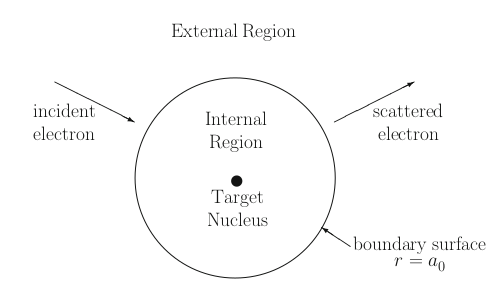
\includegraphics[width=\textwidth]{figures/theoryRM/regions.png}
\end{figure}
\end{center}
\end{column}
\begin{column}{0.45\textwidth}  %%<--- here
\begin{tikzpicture}[remember picture,overlay,
  arrow/.style={red,ultra thick,->,>=latex}]
  \tikzset{shift={(current page.center)},xshift=2.9cm,yshift=2.25cm}
  \node (target) {Estructura del blanco};
  \node (auto) at (target) [xshift=0cm,yshift=-0.65cm] {\fbox{\sc \small autostructure}};
%
  \node (inner) at (target) [xshift=0cm,yshift=-2.25cm] {Región interna};
  \node (rmatrxi) at (inner) [xshift=0cm,yshift=-0.65cm] {\fbox{\sc \small rmatrxi}};
%
  \node (outer) at (inner) [xshift=0cm,yshift=-2.25cm] {Región externa};
  \node (stgf) at (outer) [xshift=0cm,yshift=-0.65cm] {\fbox{\sc \small stgf}};
%
  \draw [arrow, bend right=0] (auto) to ([xshift=0cm,yshift=0cm]{inner.north});
  \draw [arrow, bend right=0] (rmatrxi) to ([xshift=0cm,yshift=0cm]{outer.north});
\end{tikzpicture}

\end{column}
\end{columns}


\end{frame}
%%%%%%%%%%%%%%%%%%%%%%%%%%%%%%%%%%%%%%%%%%%%%%%%%%%%%%%%%%%%%%%%%%%%%%%%
\begin{frame}
\frametitle{Descripción del blanco}

\begin{tikzpicture}[remember picture,overlay]
  \tikzset{shift={(current page.center)},xshift=0cm,yshift=1.5cm}
  \node (eqCI) 
  {$\tikzmarkin[draw=orange,fill=orange!10]{ci}(0.1,-0.4)(-0.1,0.65)
    \Phi_i(\mathbf{r}) = \sum_j c_{ji} \phi_j(\mathbf{r})
    \tikzmarkend{ci}$};
  \node (name) at (eqCI) [xshift=4.cm,yshift=0cm]
  {$\begin{array}{c}
     \mbox{\small Configuration} \\
     \mbox{\small interaction}
   \end{array}$};
  \node (pnl) at (eqCI) [xshift=0cm,yshift=-1.75cm]
   {$\left[ \frac{1}{2} \frac{d^2}{dr^2} - \frac{l(l+1)}{2r^2} 
     + V_{nl}^{\mbox{\scriptsize eff}}(\lambda_{nl},r) + E_{nl} \right] 
     P_{nl}(r)=0$};
  \node (pot) at (pnl) [xshift=-2cm,yshift=-2cm]
  {{\begin{varwidth}{\linewidth}
     \begin{itemize}
        \item Thomas–Fermi–Dirac–Amaldi 
        \item Slater-Type-Orbital de Burgess  
     \end{itemize}
    \end{varwidth}}}; 
\end{tikzpicture}

\end{frame}
%%%%%%%%%%%%%%%%%%%%%%%%%%%%%%%%%%%%%%%%%%%%%%%%%%%%%%%%%%%%%%%%%%%%%%%%
\begin{frame}
\frametitle{Ejemplo: Litio}
\begin{tikzpicture}[remember picture,overlay]
  \tikzset{shift={(current page.center)},xshift=-4cm,yshift=0cm}
  \node (licfg)
  {$\,\Vast\{ 
    \begin{array}{l}
      1s^2 2s \\
      1s^2 2p \\
      1s^2 3s \\
      1s^2 3p \\
      1s^2 3d \\
      \cdots
    \end{array}$};
  \node (lilevels) at (licfg) [xshift=5.5cm,yshift=0cm]
  {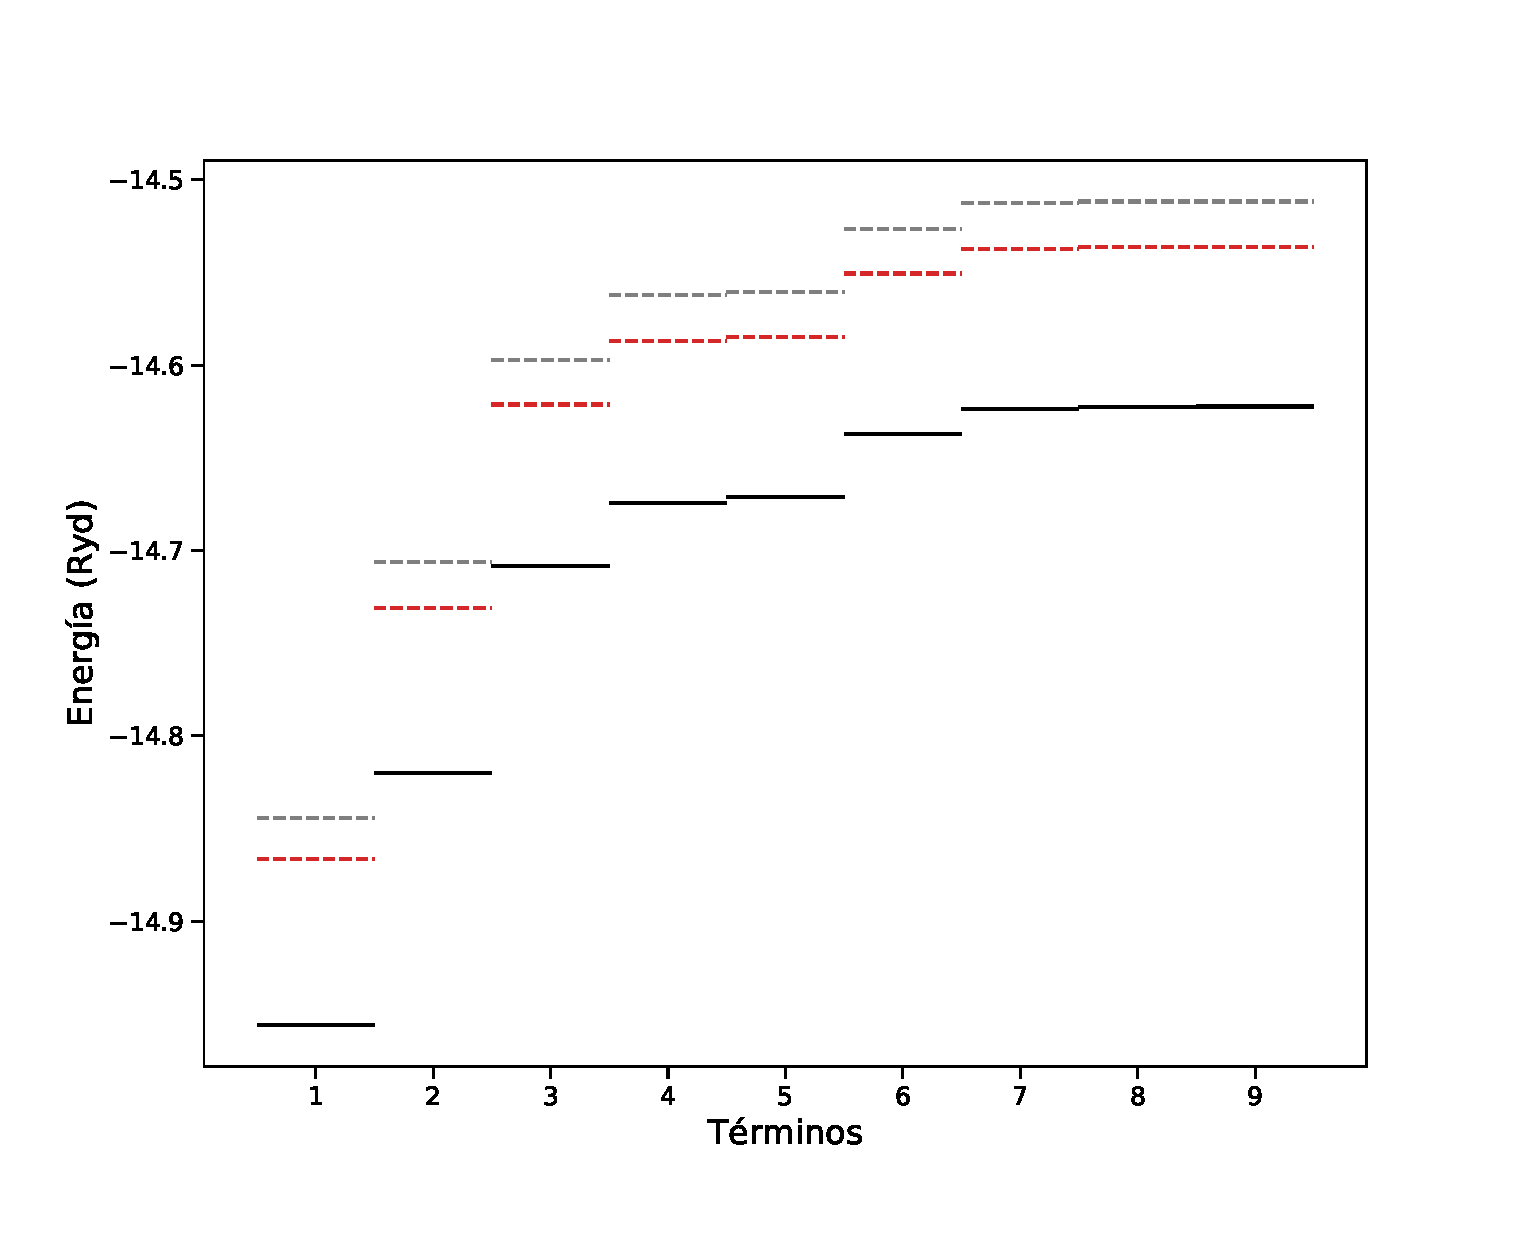
\includegraphics[width=0.7\textwidth]{figures/theoryRM/li_levels.eps}};
  \node<2-> (li) at (licfg) [xshift=5.5cm,yshift=0cm]
  {\includegraphics[width=0.7\textwidth]{figures/theoryRM/li_convergence.eps}};
\end{tikzpicture}

\end{frame}
%%%%%%%%%%%%%%%%%%%%%%%%%%%%%%%%%%%%%%%%%%%%%%%%%%%%%%%%%%%%%%%%%%%%%%%%
\begin{frame}
\frametitle{Procedimiento}

\begin{tikzpicture}[remember picture, overlay,
  expl1/.style={draw=red,fill=orange!7,rounded corners,text width=3cm,
  minimum width=0.5cm, minimum height=0.7cm, text centered},
  arrow/.style={red,ultra thick,->,>=latex}]
  \tikzset{shift={(current page.center)},xshift=0cm,yshift=1.75cm}
  \node[expl1,text width=5.3cm] (defcfg) 
  {$\begin{array}{c}
   \mbox{Definición de} \\
   \mbox{configuración electrónica} \\
    \end{array}$};
  \node[expl1,text width=2.75cm] (var) at (rem) [xshift=0cm,yshift=-1.8cm]
  {Variación de parámetros};
  \node[expl1,text width=3.1cm] (diag) at (var) [xshift=2.5cm,yshift=-2cm]
  {Diagonalización};
  \node[expl1,text width=3.3cm] (err) at (var) [xshift=-2.5cm,yshift=-2cm]
  {Calculo de error};
  \draw [arrow, bend right=0] 
  ([xshift=0cm,yshift=0cm]{defcfg}) to ([xshift=0cm,yshift=0cm]{var.north});
  \draw [arrow, bend right=-30] 
  ([xshift=0cm,yshift=0cm]{var.east}) to ([xshift=0cm,yshift=0cm]{diag.north});
  \draw [arrow, bend right=-40] 
  ([xshift=0cm,yshift=0cm]{diag}) to ([xshift=0cm,yshift=0cm]{err.south});
  \draw [arrow, bend right=-30] 
  ([xshift=0cm,yshift=0cm]{err}) to ([xshift=0cm,yshift=0cm]{var.west});
  \draw [arrow, bend right=-30,dashed] 
  ([xshift=-0.75cm,yshift=0cm]{err.north}) to ([xshift=0cm,yshift=-0.25cm]{defcfg.west});
\end{tikzpicture}

\end{frame}
%%%%%%%%%%%%%%%%%%%%%%%%%%%%%%%%%%%%%%%%%%%%%%%%%%%%%%%%%%%%%%%%%%%%%%%%
\begin{frame}
\frametitle{Síntesis del problema}

\begin{equation*}
 J = \sum_j \left|\frac{E_j^{\mbox{\small calc}}(\boldsymbol{\xi}) 
- E_j^{\mbox{\small teo}}}{E_j^{\mbox{\small teo}}} \right|
\end{equation*}

\medskip
\begin{itemize}
\item DIM: $\boldsymbol{\xi}=\{\boldsymbol{\alpha},\boldsymbol{\beta} \}$
\item R--Matrix: $\boldsymbol{\xi}=\{ Configuraciones,\boldsymbol{\lambda} \}$
\end{itemize}

\end{frame}
%%%%%%%%%%%%%%%%%%%%%%%%%%%%%%%%%%%%%%%%%%%%%%%%%%%%%%%%%%%%%%%%%%%%%%%%
\begin{comment}

\begin{tikzpicture}[remember picture, overlay]
  \tikzset{shift={(current page.center)},xshift=0cm,yshift=2.25cm}
  \node (eq0) 
  {$\left[ \frac{1}{2} \frac{d^2}{dr^2} - \frac{l(l+1)}{2r^2} 
     + V_{\mbox{\scriptsize eff}}(r) + \epsilon_{nl} \right] 
     P_{nl}(r)=0$};
  \node<-1> (pot) at (eq0) [xshift=-2cm,yshift=-3.75cm]
  {
    {\begin{varwidth}{\linewidth}
%     Potencial modelo:
     \begin{itemize}
        \item Thomas–Fermi–Dirac–Amaldi 
          $$ V(\lambda_{nl},r) = $$
        \item Slater-Type-Orbital de Burgess  
          $$ V(\lambda_{nl},r) = $$
     \end{itemize}
     \end{varwidth}}}; 
\end{tikzpicture}

  \node<2-> (fun) at (eq0) [xshift=-0.1cm,yshift=-4cm]
  {
    {\begin{varwidth}{\linewidth}
     Funciones de onda:
     \begin{itemize}
        \item Estados espectroscópicos:
\vspace{-0.3cm}
          $$  P_{nl}(r)=\sqrt{\frac{(2\lambda_{\text{nl}})^{2I_{\text{nl}}+1}}{\left(2 I_{\text{nl}}\right)!}}\, r^{I_{\text{nl}}} 
   e^{-\lambda_{\text{nl}}r} $$
\vspace{-0.7cm}
        \item Pseudo--estados:
\vspace{-0.2cm}
          $$  P_{nl}(r) = N_{nl}\,(\lambda_{nl} Z r)^{l+1} \,e^{-\lambda_{nl}Zr/2} \,
 L_{n+l}^{2l+1}(\lambda_{nl} Z r) $$
     \end{itemize}
     \end{varwidth}}}; 
\end{comment}
%%%%%%%%%%%%%%%%%%%%%%%%%%%%%%%%%%%%%%%%%%%%%%%%%%%%%%%%%%%%%%%%%%%%%%%%
\begin{frame}
\frametitle{Procesos Gaussianos}

\begin{tikzpicture}[remember picture, overlay]
  \tikzset{shift={(current page.center)},xshift=0cm,yshift=-0.5cm}
  \node<1> (prior) {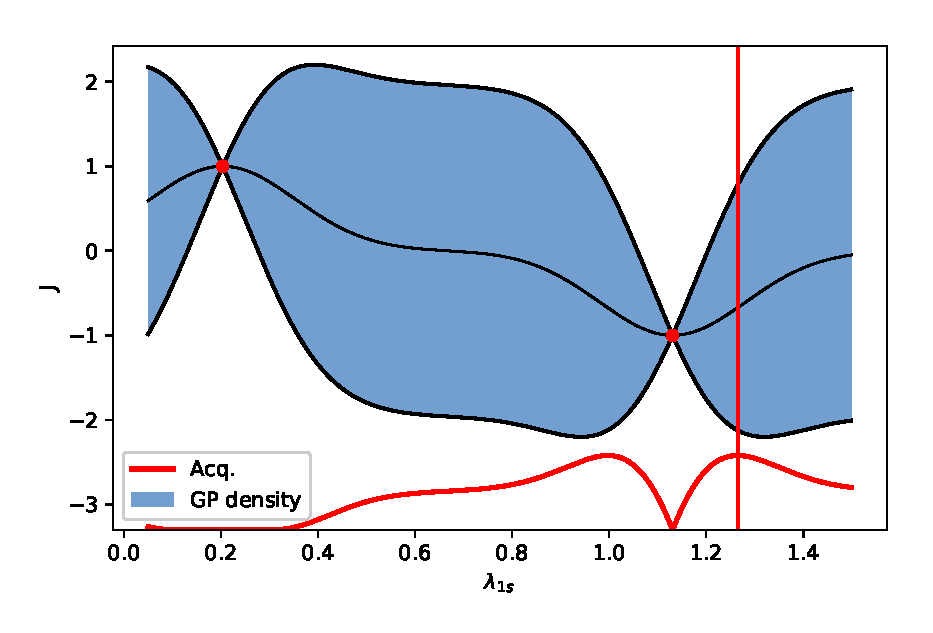
\includegraphics[width=0.9\textwidth]{figures/gp/lam1s_init2.eps}};
  \node<2> (max1) {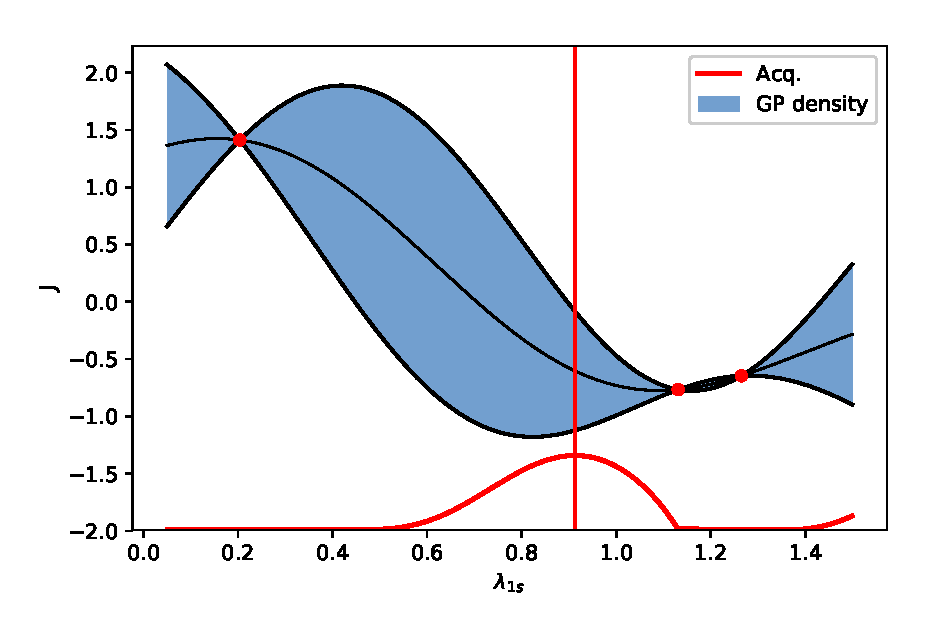
\includegraphics[width=0.9\textwidth]{figures/gp/lam1s_init2_maxevals1.eps}};
  \node<3> (max2) {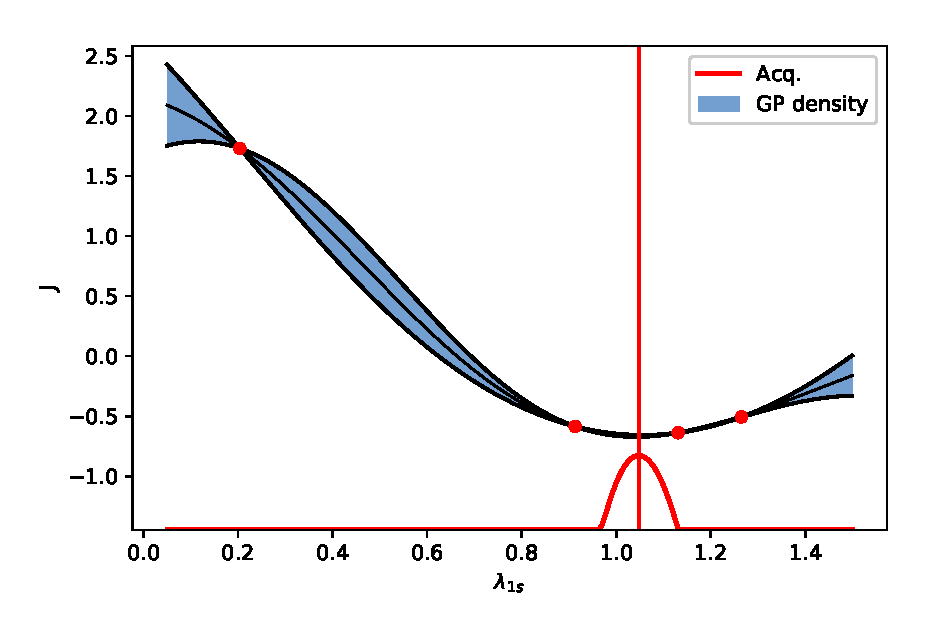
\includegraphics[width=0.9\textwidth]{figures/gp/lam1s_init2_maxevals2.eps}};
  \node<4> (max3) {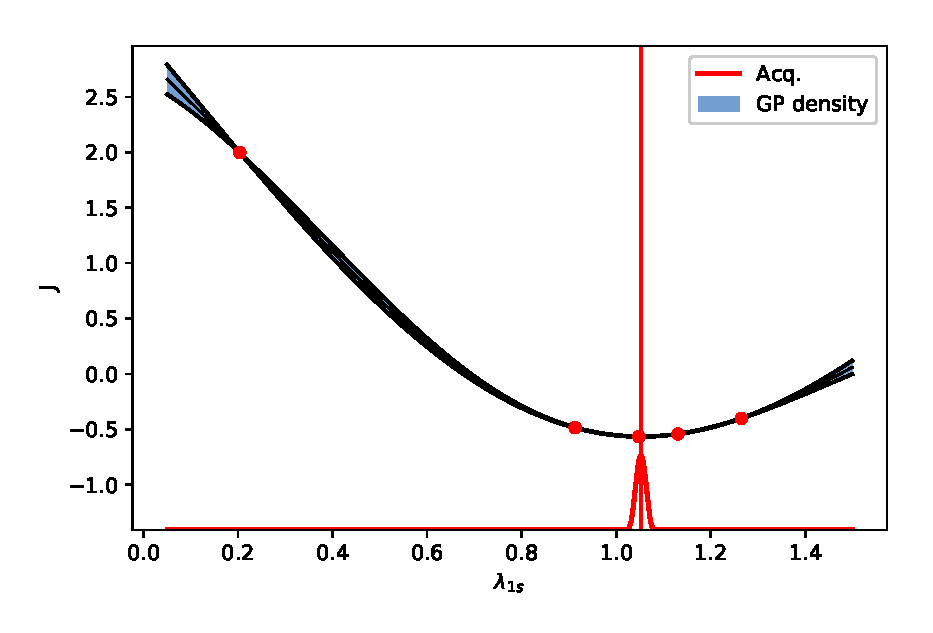
\includegraphics[width=0.9\textwidth]{figures/gp/lam1s_init2_maxevals3.eps}};
\end{tikzpicture}
\end{frame}
%%%%%%%%%%%%%%%%%%%%%%%%%%%%%%%%%%%%%%%%%%%%%%%%%%%%%%%%%%%%%%%%%%%%%%%%
\section{Resultados}
%%%%%%%%%%%%%%%%%%%%%%%%%%%%%%%%%%%%%%%%%%%%%%%%%%%%%%%%%%%%%%%%%%%%%%%%
\begin{frame}
\frametitle{Resultados DIM}

\end{frame}
%%%%%%%%%%%%%%%%%%%%%%%%%%%%%%%%%%%%%%%%%%%%%%%%%%%%%%%%%%%%%%%%%%%%%%%%
\begin{frame}
\frametitle{Resultados R--Matrix}

\vspace{-0.2cm}
\begin{figure}
\includegraphics[width=0.4\textwidth]{figures/rmatrix/sig001-002.eps}
\includegraphics[width=0.4\textwidth]{figures/rmatrix/sig001-003.eps} \\
\vspace{0.2cm}
\includegraphics[width=0.4\textwidth]{figures/rmatrix/sig001-006.eps} 
\includegraphics[width=0.4\textwidth]{figures/rmatrix/sig001-007.eps}
\end{figure}

\end{frame}
%%%%%%%%%%%%%%%%%%%%%%%%%%%%%%%%%%%%%%%%%%%%%%%%%%%%%%%%%%%%%%%%%%%%%%%%
\end{document}
